\section{Scenario's}
De scenario view is een representatie van de belangrijkste use cases van het systeem \parencite{4+1ViewModelPaper}.
De use cases zijn opgesteld door middel van de geprioriteerde lijst van requirements van het onderzoek \parencite{DanteOnderzoek}.
Om de verschillende use cases en interactie met andere actoren in het systeem in beeld te krijgen wordt er gebruik gemaakt van een use case diagram \parencite{UseCaseDiagram}.
In figuur \ref{fig:UseCaseDiagramCMS(1)}, \ref{fig:UseCaseDiagramCMS(2)} en \ref{fig:UseCaseDiagramBekijkenVanContent} zijn de verschillende use case diagramen te zien.
Er is voor gekozen om de use cases voor het CMS-platform op te delen om het meer overzichtelijk te maken.

\whitespace[2]
\begin{graphic}
	\captionsetup{type=figure}
	\caption{Use case diagram CMS(1)}
	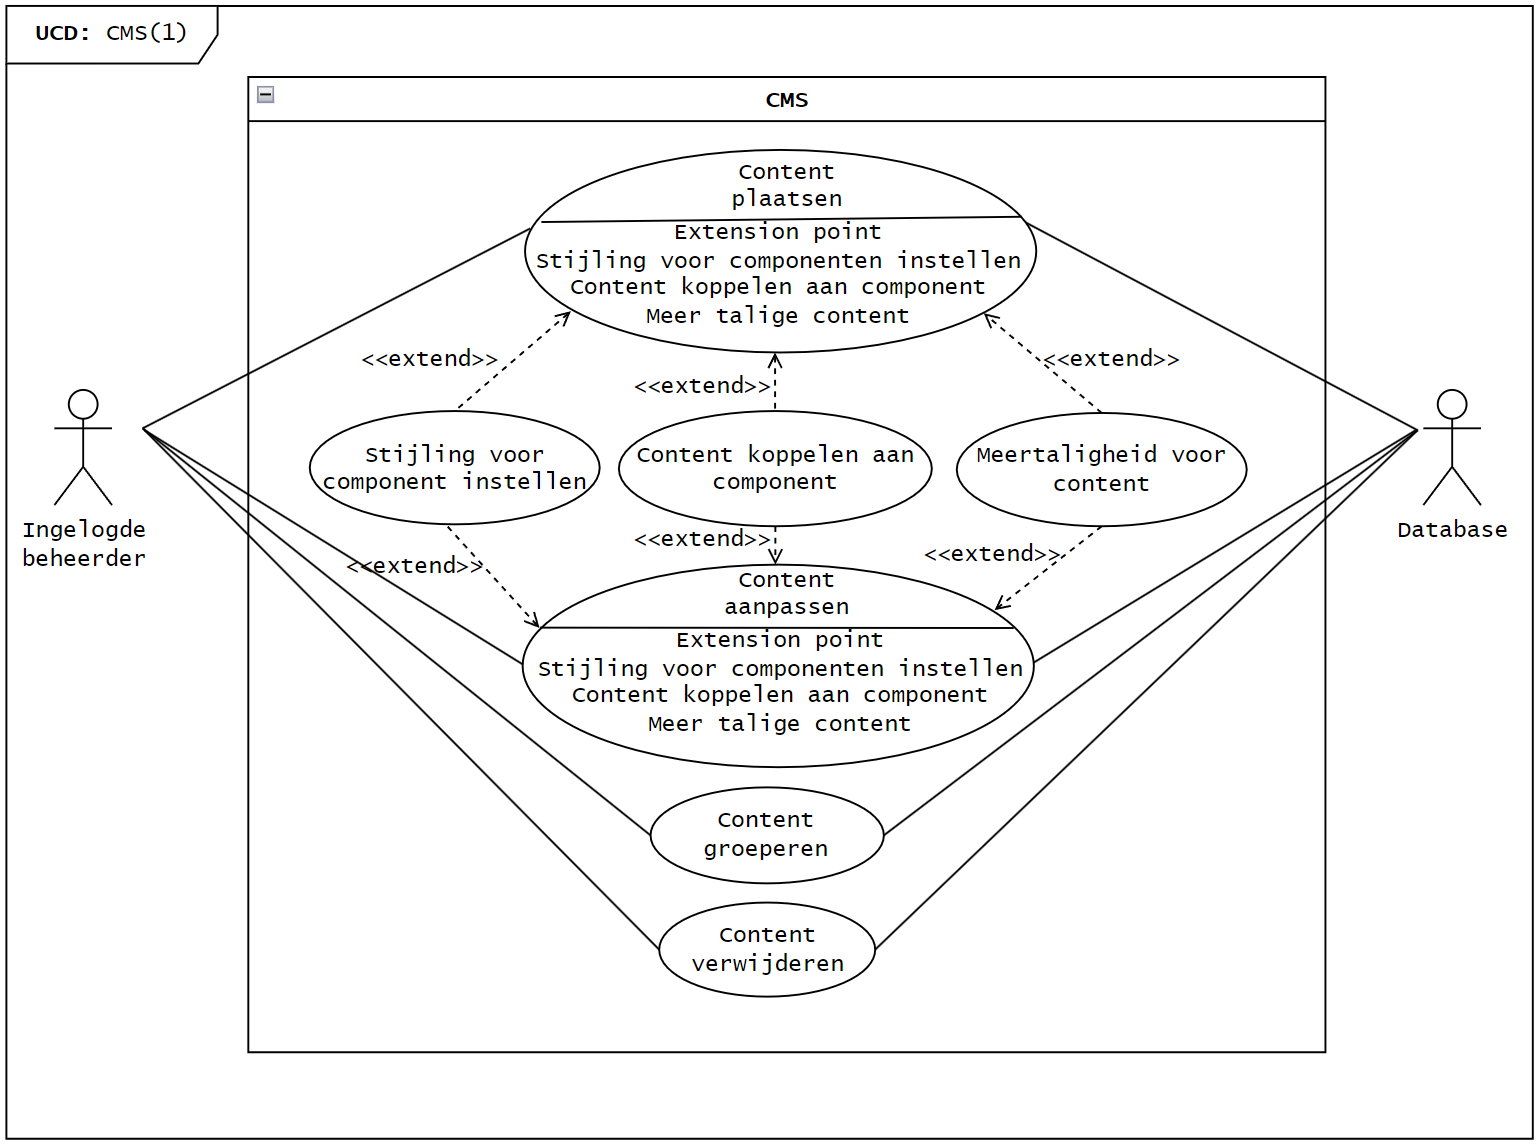
\includegraphics[scale=0.45]{UseCaseDiagramCMS(1).png}
	\label{fig:UseCaseDiagramCMS(1)}
\end{graphic}

\whitespace[2]
In figuur \ref{fig:UseCaseDiagramCMS(1)} zijn de verschillende use cases te zien die te maken hebben met de content binnen het CMS.
Voor de overige functionaliteiten is er in figuur \ref{fig:UseCaseDiagramCMS(2)} ook een use case diagram te vinden.
Dit use case diagram toont het authenticatie en algemene site functionaliteit.
Het laatste diagram (figuur \ref{fig:UseCaseDiagramBekijkenVanContent}) is gemaakt voor de klanten site.
Dit is de locatie waar de (website) bezoeker de content kan bekijken.

\newpage
\begin{graphic}
	\captionsetup{type=figure}
	\caption{Use case diagram CMS(2)}
	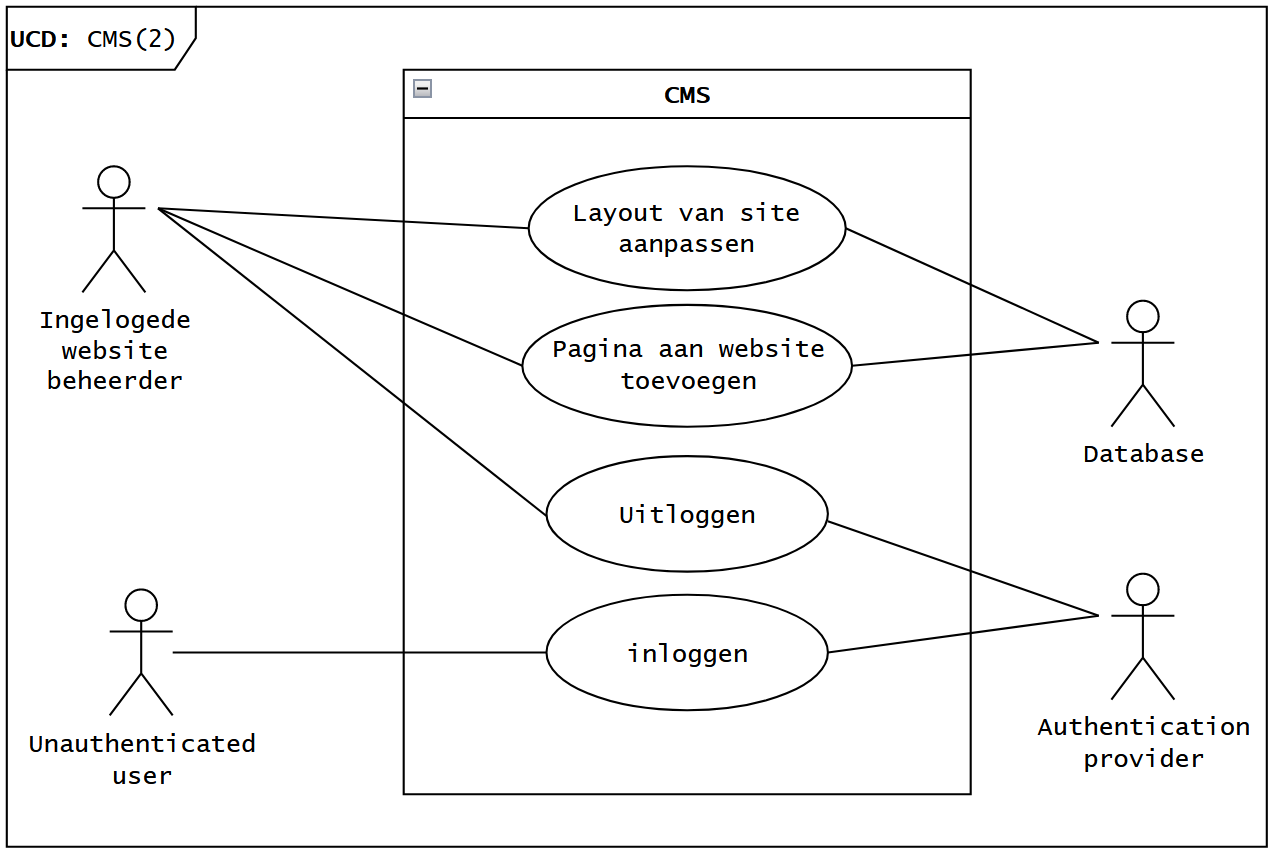
\includegraphics[scale=0.4]{UseCaseDiagramCMS(2).png}
	\label{fig:UseCaseDiagramCMS(2)}
\end{graphic}

\whitespace
\begin{graphic}
	\captionsetup{type=figure}
	\caption{Use case diagram klant site}
	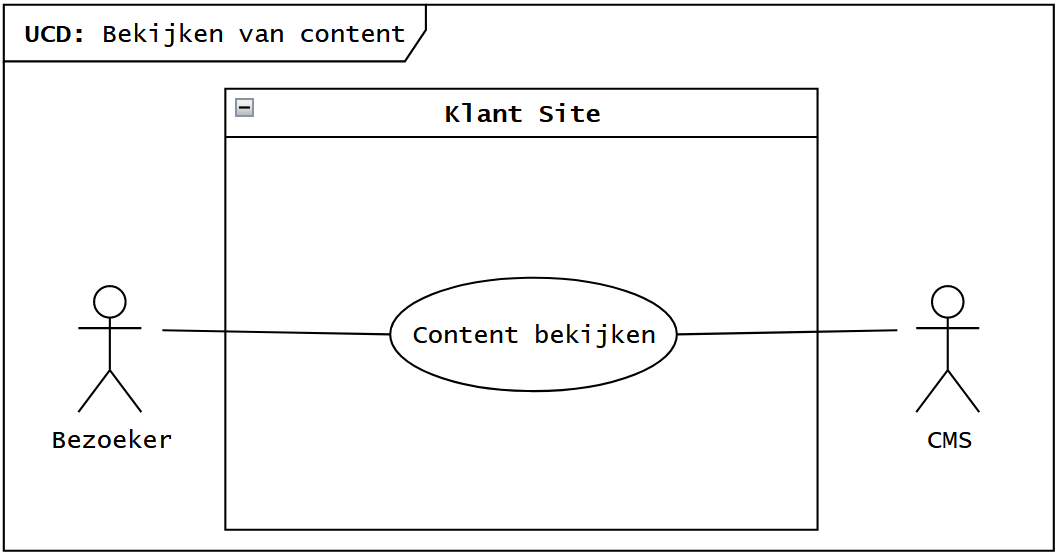
\includegraphics[scale=0.4]{UseCaseDiagramBekijkenVanContent.png}
	\label{fig:UseCaseDiagramBekijkenVanContent}
\end{graphic}
